\documentclass[12p]{article}
\usepackage[margin=1in, headheight=110pt]{geometry}
\usepackage{amssymb, amsmath, amsfonts, amsthm}
\usepackage{mathpazo}
\usepackage{setspace}
% \usepackage{probsoln}
\usepackage{fancyhdr}
\usepackage{hyperref}
\usepackage{float}
\usepackage{tikz}
\usepackage{enumitem}
\usepackage{graphicx}
\usepackage{listings}
\usepackage{caption}
\usepackage{bookmark}

\def\ojoin{\setbox0=\hbox{$\bowtie$}%
  \rule[-.02ex]{.25em}{.4pt}\llap{\rule[\ht0]{.25em}{.4pt}}}
\def\leftouterjoin{\mathbin{\ojoin\mkern-5.8mu\bowtie}}
\def\rightouterjoin{\mathbin{\bowtie\mkern-5.8mu\ojoin}}
\def\fullouterjoin{\mathbin{\ojoin\mkern-5.8mu\bowtie\mkern-5.8mu\o}}

\pagestyle{fancy}
\lhead{Team 2}
\rhead{SENG 300 - Group Project Iteration 2 - Winter 2018}
\title{\vspace{-6ex}Groupd Project Iteration 2}
\date{\vspace{-12ex}}


\newcommand{\code}[1]{\texttt{#1}}

\setlength{\parindent}{0pt}
\begin{document}
% \maketitle
\thispagestyle{fancy}

\begin{titlepage}
  \begin{center}
    \vspace{1cm}
    \Large{\textbf{University of Calgary}}\\
    \Large{\textbf{SENG 300  - Introduction to Software Engineering}}
    \vfill
    \line(1,0){400}\\[1mm]
    \huge{Group Project Iteration 2}\\
    \large{Finding Declarations and References}\\
    \line(1,0){400}\\
    \Large March 26, 2018\\
    \vfill
    \huge{Team 2}\\
    \Large
    Evan Quan 10154242\\
    Marcello Di Benedetto 30031839\\
    Mona Agh 30033301\\
    Sunah Kim 10155604\\
    Zahra Al Ibrahim 30020048\\
  \end{center}
\end{titlepage}

% \tableofcontents
% \thispagestyle{empty}
% \clearpage
%
% \onehalfspacing
%
% \setcounter{page}{1}

\section{Structural Diagram}
\begin{figure}[H]
  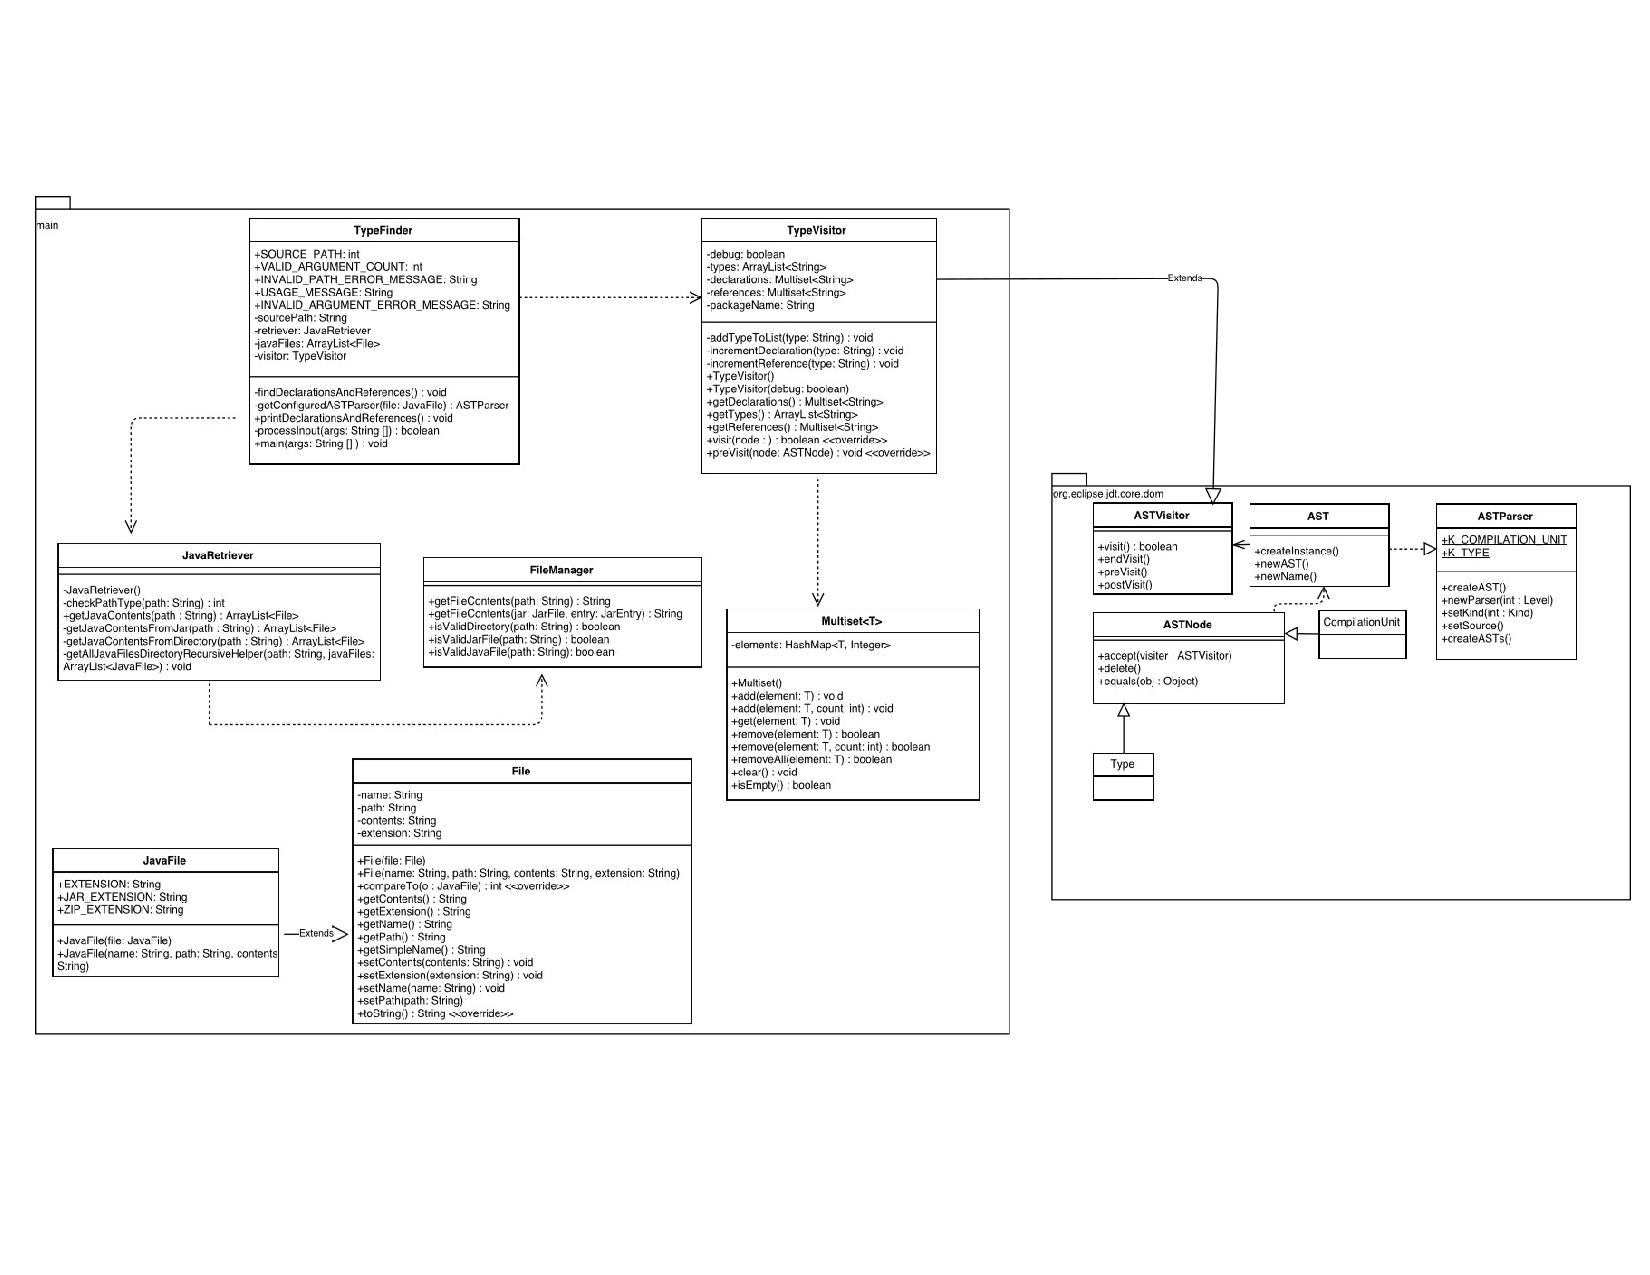
\includegraphics[width=1.00\textwidth]{StructuralDiagramIteration_2.pdf}
  \caption{The relationship between our main package and relevant classes provided by org.eclipse.jdt.core.dom. TypeFinder acts as the main class that handles user input, manages other classes, and output results. JavaRetriever retrieves Java file contents from the directory or .jar of choice. TypeVisitor counts the references and declarations from the Java file contents.} % TODO caption
  \label{fig:structural}
\end{figure}


\section{Sequence Diagrams}

\begin{figure}
  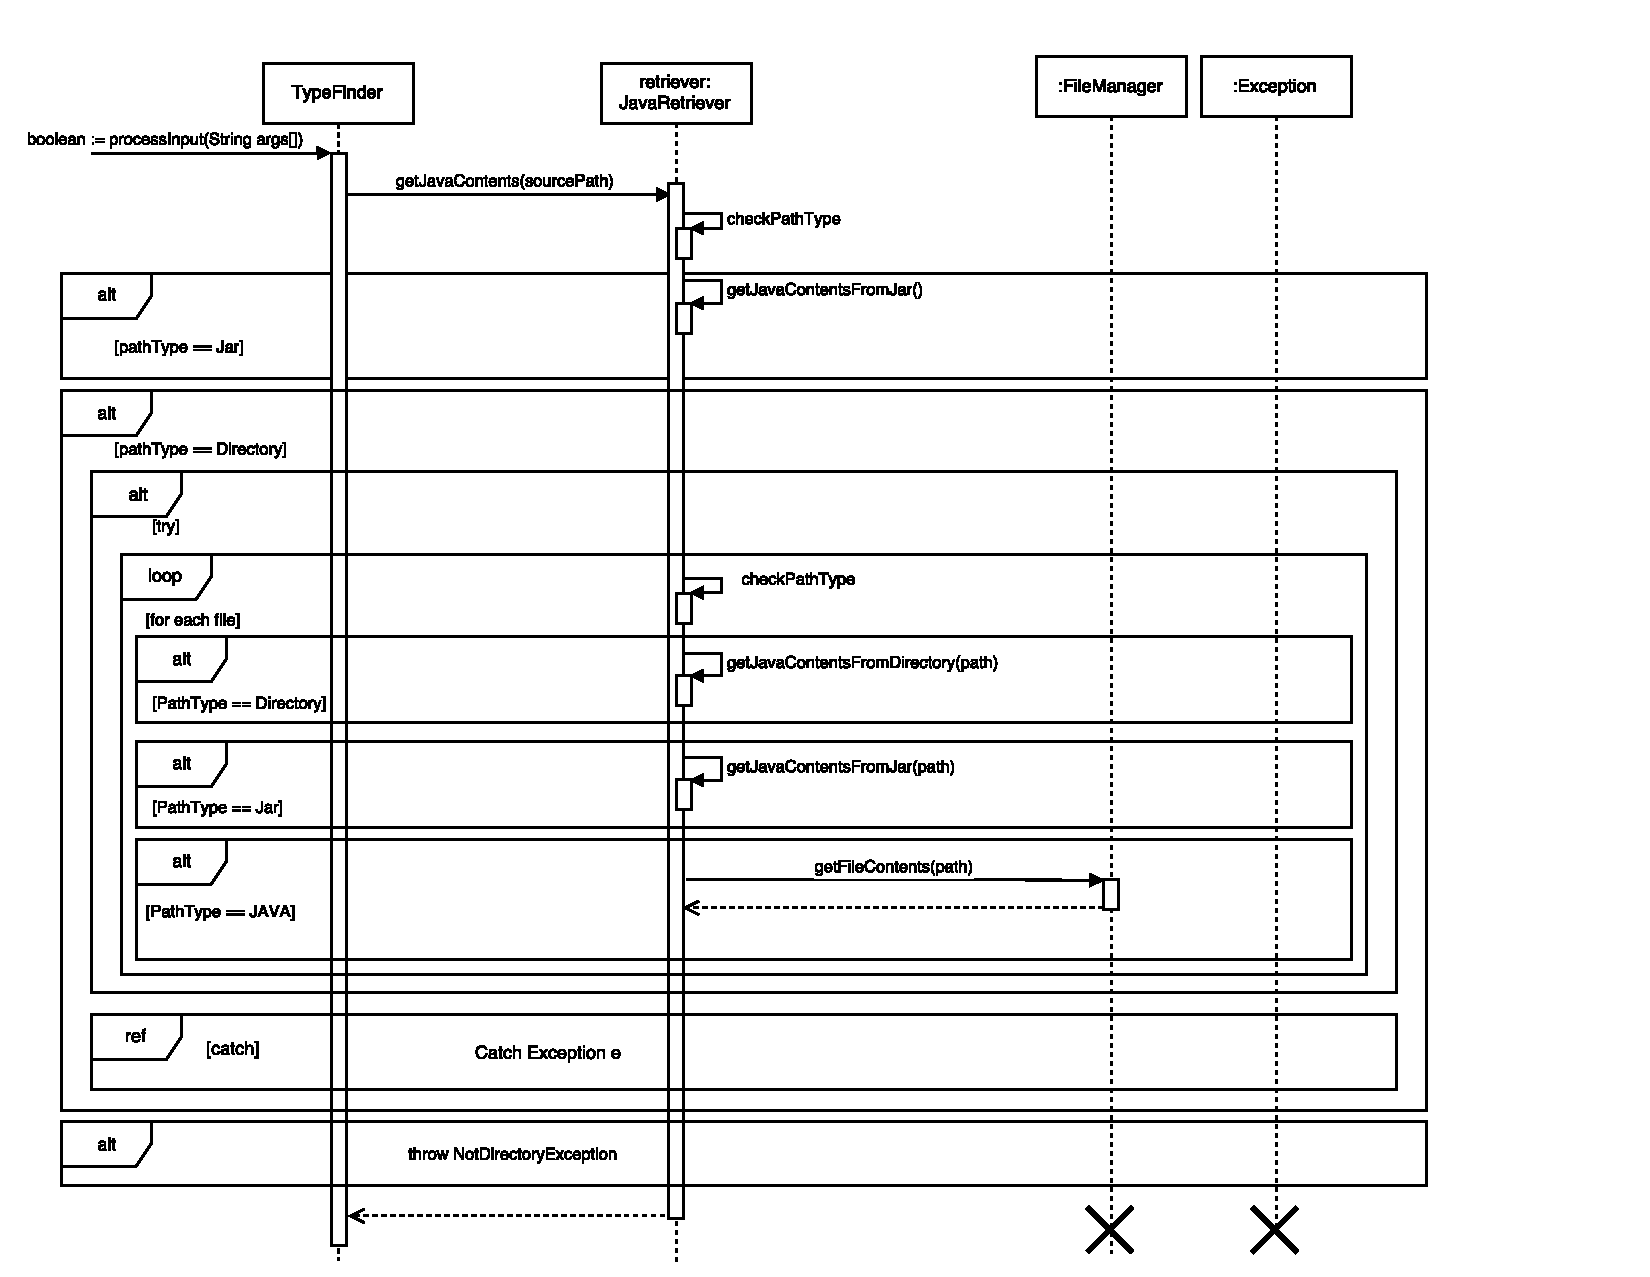
\includegraphics[width=1.0\textwidth]{JavaRetriever-Iteration2.pdf}
  \caption{Sequence of JavaRetriever retrieving the contents of all Java files in a directory or .jar file recursively, so it can be later processed to find the references and declarations.} % TODO caption
  \label{fig:sequence2}
\end{figure}

\begin{figure}[H]
  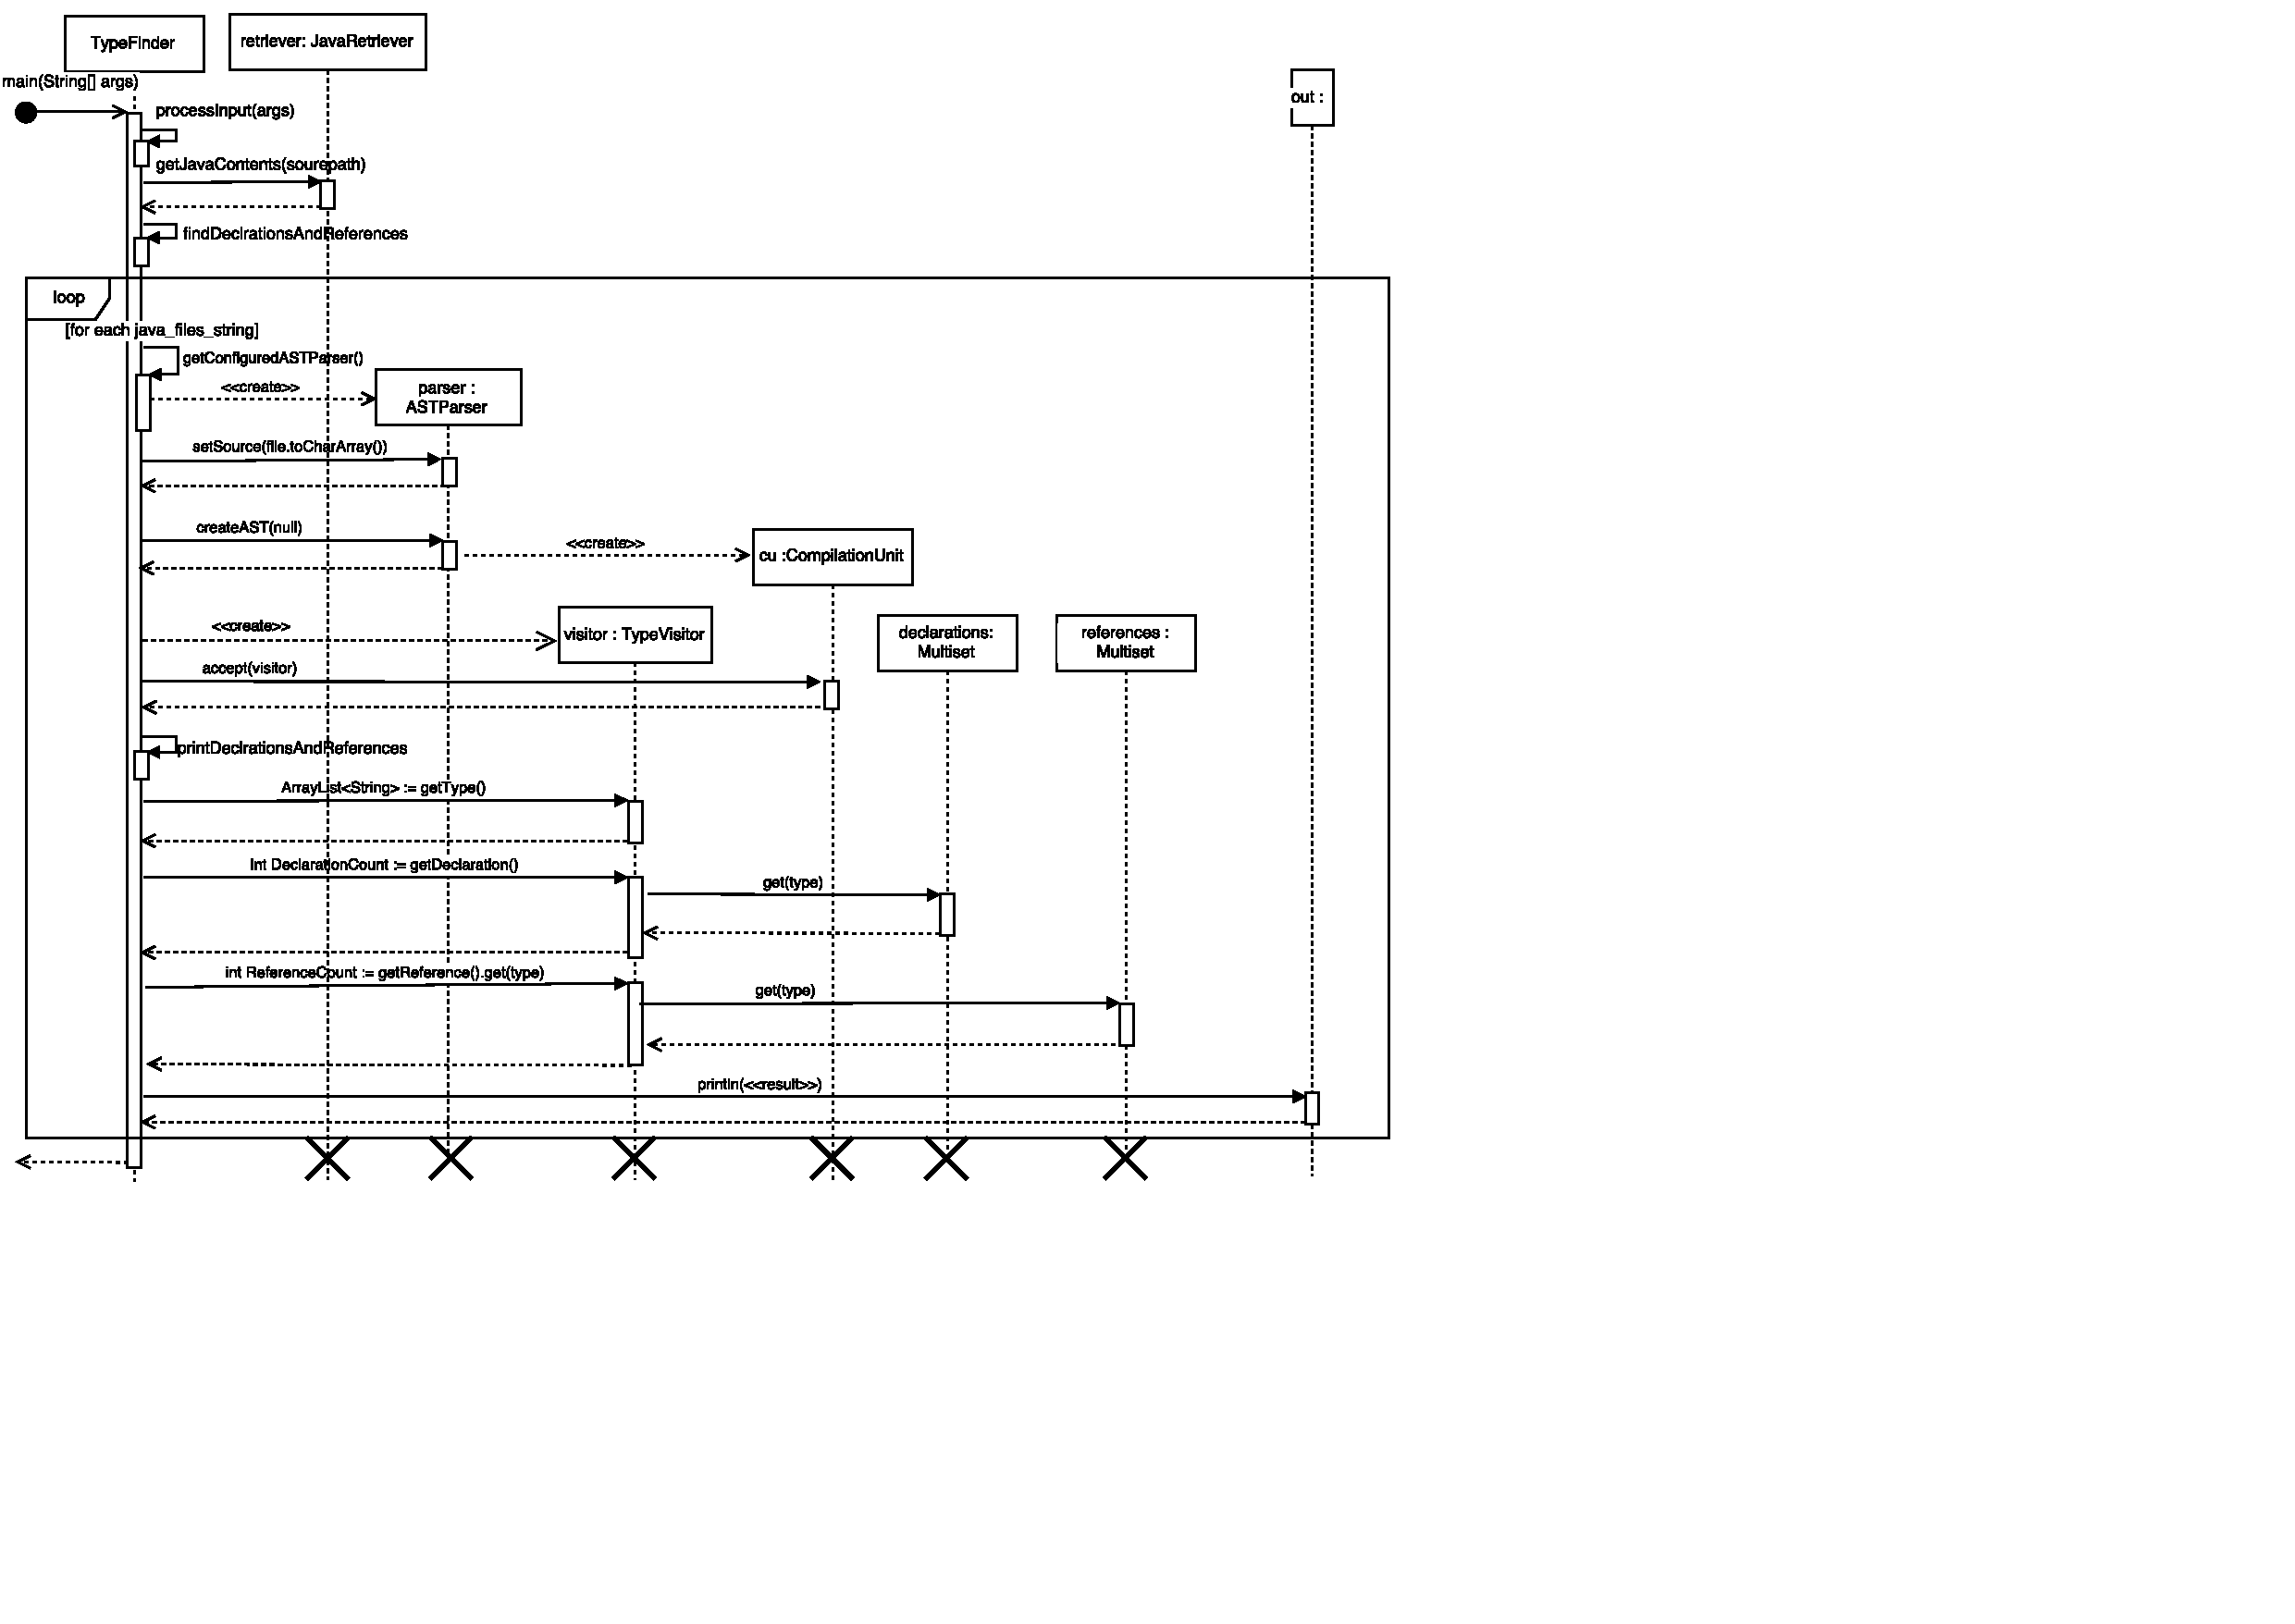
\includegraphics[width=1.00\textwidth]{mainTypeFinder-Iteration2.pdf}
  \caption{Sequence of TypeFinder program intialization and completion, emphasizing how the program processes finding the reference and declaration counts after the Java file contents have been acquired.} % TODO caption
  \label{fig:sequence1}
\end{figure}


\newpage

\section{State Diagram}
\begin{figure}[H]
  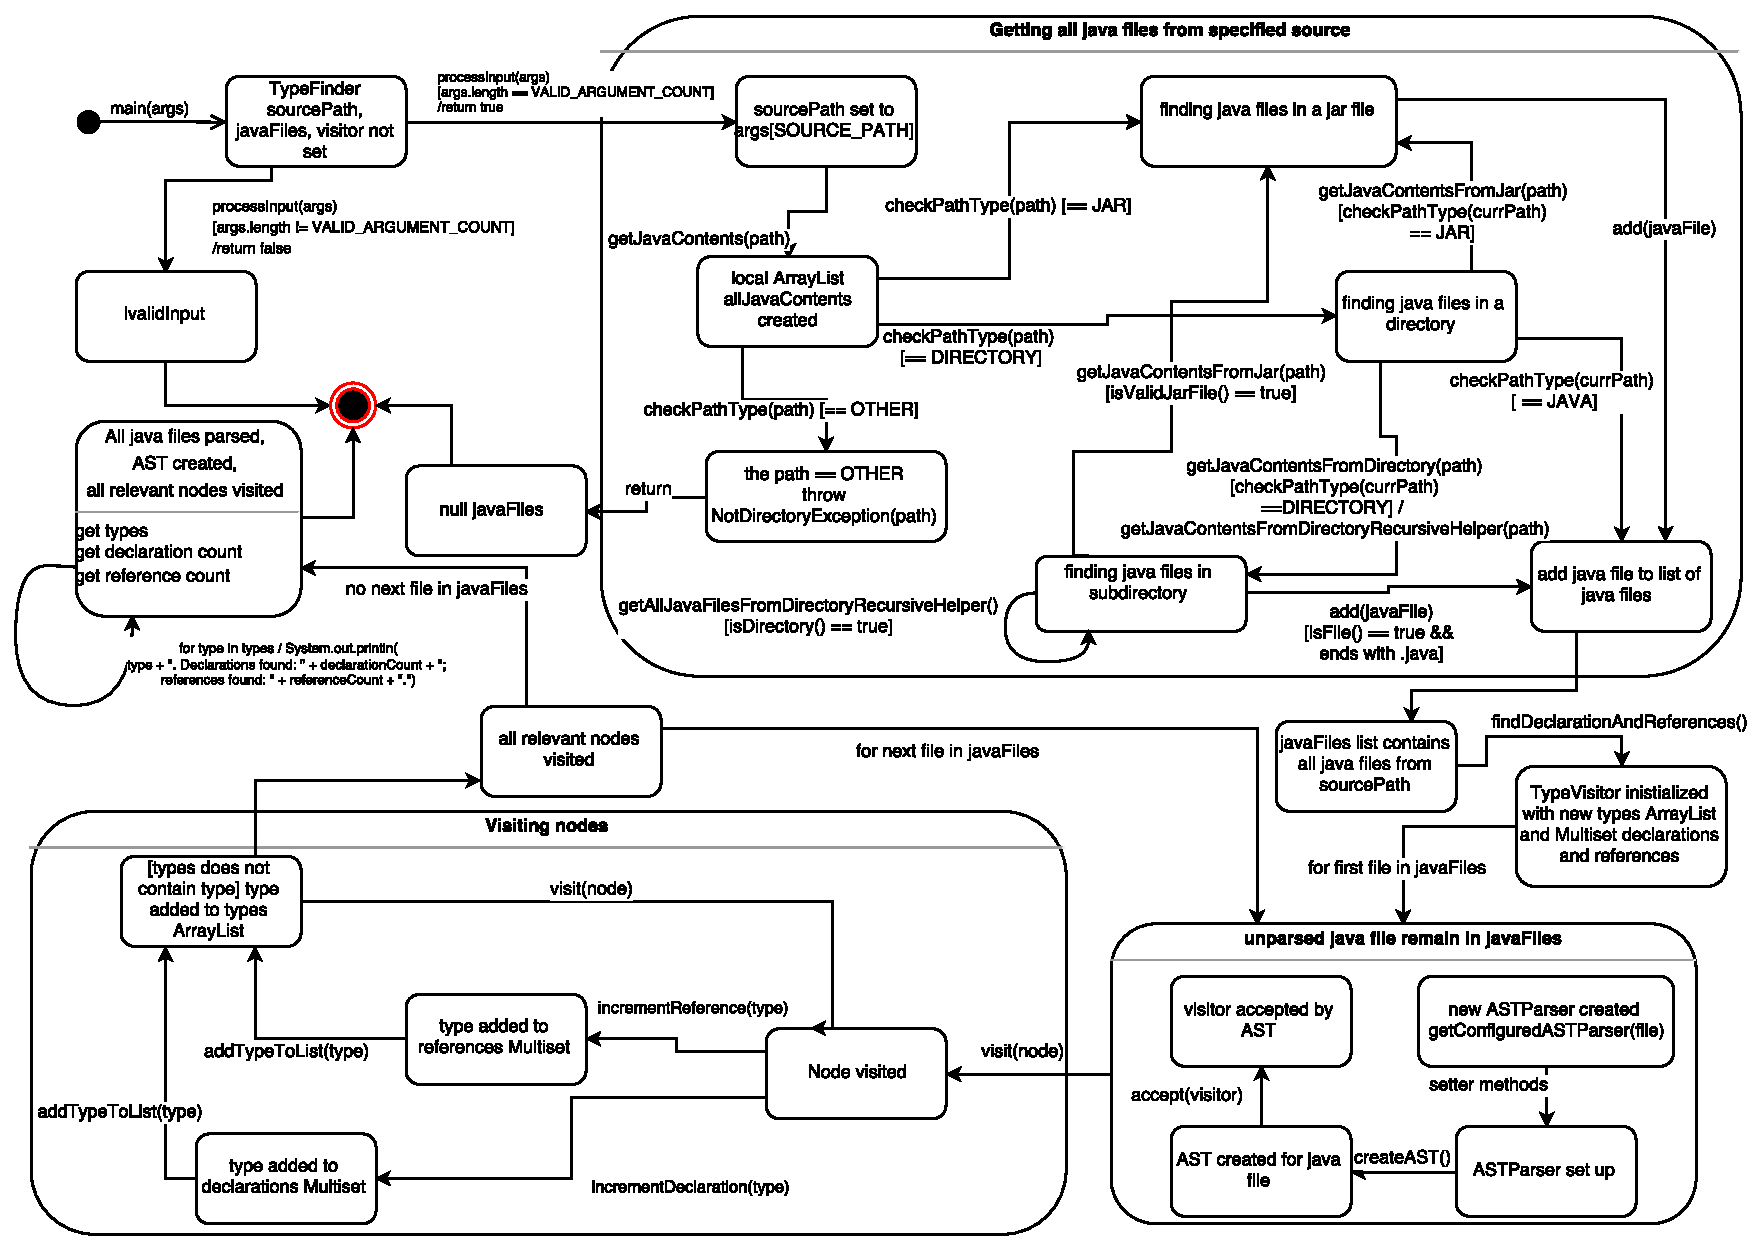
\includegraphics[width=1.0\textwidth]{StateDiagram_Iteration2.pdf}
  \caption{The state of the program in finding declaration and reference counts.} % TODO caption
  \label{fig:state}
\end{figure}

\newpage
\section{Explanation}
\subsection{Program description}
This program finds all Java types all .java files in a directory and all subdirectories (recursively) or .jar file and outputs to the console the type name and with the number of declarations and references of each type.
It makes use of classes in the org.eclipse.core.dom package such as the ASTParser in order to parse a .java file, from which an AST is created.
The declarations and references of Java types are found visiting specific nodes of the AST through an ASTVisitor.

\subsection{Usage}
Run the Java \code{TypeFinder.class} file through command line:

\code{java TypeFinder <path of directory or jar>}

\subsection{Structure}
% The UML diagram was kept as simple as possible and only represent main components of the software. All the methods in the Type Finder Class were included since they drive the software during execution. The JavaFileReader class is reads the all files in the directory and allows for parsing via AST. We Did not include all the methods for the TypeVisitor. The abstracted details were only supporting features that did not aid in the understanding of the functionality. As for visit (node : ) : boolean, the formatting was done this way due to the multiple overridden methods with different parameter types, such as SingleVariableDecleration, TypeDecleration...etc.
% like the rest only the key components of the ASTParser, AST, ASTVistor, ASTNode were maintained in the Uml Diagram. Everything that did not aid or was none essential in understanding the relationships between the TypeFinder and the AST parser was left out.
The UML diagram shows the important components of the software. Most of the methods in the TypeFinder class were represented in the diagram since they drive the software during execution. The classes JavaRetriever, JavaFile, File, and FileMangaer are used to read files and get their contents so that we can parse the files. Because of that, it was essential to represent those. Multiset$<$T$>$ was used to store the declarations and references found. Therefore, the TypeVisitor class depends on it. We did not include all the methods for the TypeVisitor. The abstracted details were only supporting features that did not aid in the understanding of the functionality. As for visit (node : ) : boolean, the formatting was done this way due to the multiple overridden methods with different parameter types, such as SingleVariableDecleration, TypeDecleration...etc. like the rest only the key components of the ASTParser, AST, ASTVistor, ASTNode were maintained in the Uml Diagram. Everything that did not aid or was none essential in understanding the relationships between the TypeFinder and the AST parser was left out.

\subsection{Sequence Diagram}
% The software works by receiving arguments from the user, those being the directory of interest and the fully qualified name of a java type. It the enters a loop which executes per file read. After entering the loop, the ASTParser is configured with the correct specifications and created. after that the file to be read is set and the AST is created along with a visitor. we then begin to visit the nodes of the AST counting the number of declaration/references of types. finally, at the end of the loop we sum the total number of counts. the loop is exited and the number of references and declarations in printed to the console.
% The inner workings of the getConfiguredASTParser () method is non-essential to the client's understanding of the software. Thus, the details were abstracted away and not expanded on. Another aspect of the code that was abstracted away was most of the methods in JavaFileReader. We modeled a very broad overview, this informs anyone viewing the model (provided some basic knowledge of java) of what is happening. Had we made our diagram anymore specific in this area, it would draw attention away from the more important functionality of the software and would only overwhelm the viewer. A very basic diagram shows the execution of initFinder, which was only meant to serve the purpose of showing that the javaFileReader Class was being used to read the files. A more Specific sequence diagram was provided to show how getAllJavaFilesToStrings () was receiving information about the directory and files, as well as how it returned the result for ASTParser to use.
The sequence diagram for this software has shown in two separate diagrams. The first one depicts an overall view of how the software works. It first start by receiving the argument from the user which is the pathname of a directory or JAR file and check if the arguments is valid. Then, it calls an instance of JavaRetriever class which has the responsibility of iteration through the directory or JAR files recursively and reading all Java files. After that, it enters into a loop which creates ASTParser for each Java files, sets the configuration and create AST as CompilationUnit. Following from last step, it creates a visitor to visit each node of the AST and count the number of declaration and references for each node and finally, print the result for all types on the console. The second diagram show in more detail how the software recursively goes through the directory or JAR files of given pathname. It checks the pathname of interest to find its type, and cording to that, if it's a directory, a JAR file or a Java file takes the appropriate action. We used abstraction and we did not show all the details in the diagram specifically the steps that it takes to read the content of files to make easier for the client to understand the functionality of the software.

\subsection{State diagram}
% The state diagrams show the transition of states while visiting the nodes. While visiting a node you can update the type list, once the list is either updated or not updated then then the count is incremented if the type is found.  Continuing this cycle of visiting and checking nodes until there are no more nodes to analyze,   the visiting state is left  return to the loop at main in TypeFinder. Again, many details were abstracted away to reduce clutter and confusion. the main purpose was to aid in the understanding of functionality and execution of analysis tool.
The diagram is divided into three major states: 1) Getting java files, where the states are based on the path type (directory, jar, java, other) that the program is looking at. 2) Parsing Java file, where states are based on setting up/using ASTParser and creating AST. 3) Visiting nodes for each AST created to get declarations and references of types. The program reaches the end after all files are parsed, ASTs created for each parsed file, all relevant nodes visited for each AST, and all types with declaration and reference count are printed.

\end{document}
